\section{Permanent set model results}
\subsection{Model fit and predictive capabilities}


	For the strain control specimens, we found that we were able to fit the permanent set deformations very well ($R^2 = 0.96$) (Fig. \ref{fig:strainresults}A). We were able to predict the mechanical response of the strain controlled specimens at 65 million cycles ($R^2 = 0.83$) (Fig. \ref{fig:strainresults}B\&C). 
	For the stress controlled specimens, we found we were able to fit the permanent set deformations for the XD specimens ($R^2 = 0.93$)(Fig. \ref{fig:stressXDdef}B), as well as predict the PD specimens very well ($R^2 = 0.97$) (Fig. \ref{fig:stressXDdef}C). 
	The resulting rate constant from both data sets shown no statistical difference ($p > 0.98$)(Fig. \ref{fig:stressXDdef}A). 
The mechanical response for the stress controlled XD specimens did not match as well in terms of the $R^2$ value($R^2 = 0.72$). 
	However, given none of the mechanical data was involved in the parameter estimate this was nevertheless a very good prediction. 
	For example, when comparing the model to the experimental data by extrapolating the loading path of the equibiaxial protocol and finding the peak strain at 1MPa, the $R^2$ value increases to 0.93. 
	One the other hand, the predicted mechanical response for the PD controlled data were very good ($R^2 = 0.95$) (Fig. \ref{fig:stressPDmech}), suggesting that our model was able to capture the underlying mechanisms. 
	These results agree with our hypothesis that the initial changes in the mechanical response (in the first 50 million cycles) can be predicted by the change in microstructure alone, and that structural damage is low at this stage. 
\begin{figure}[hbt]
\centering
\centerline{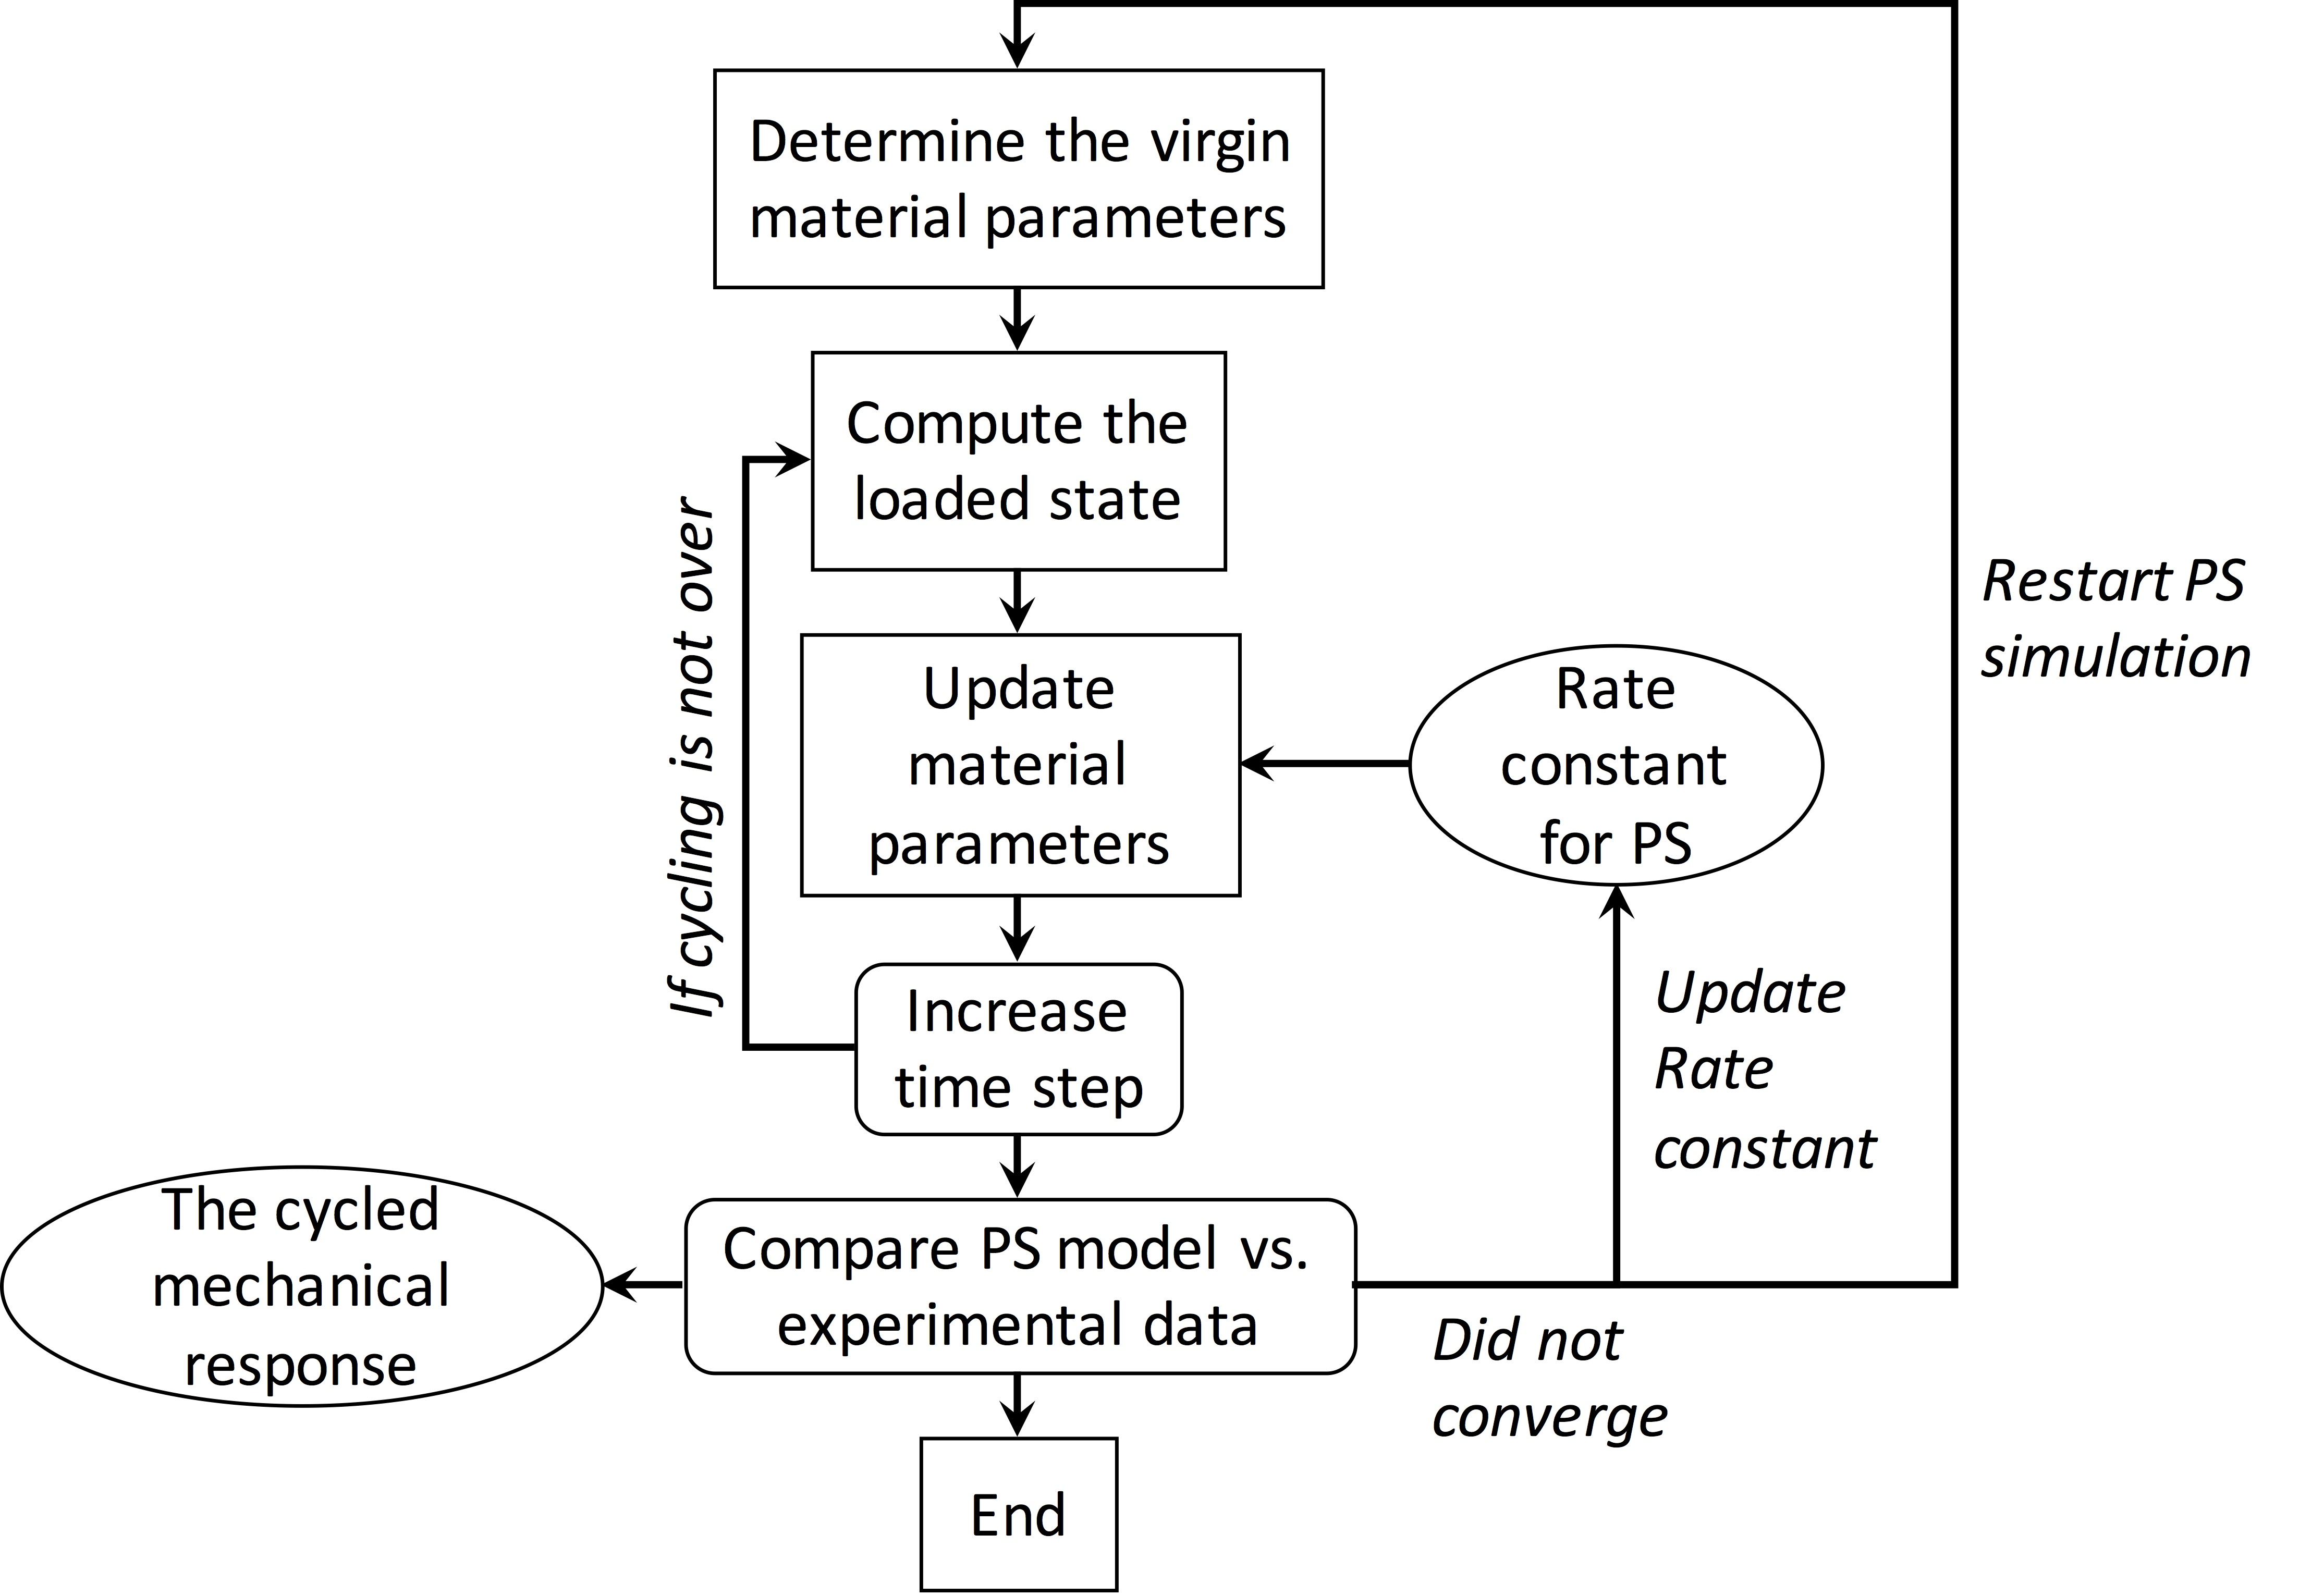
\includegraphics[width=0.75\paperwidth]{Images/chapter4/figure13}}
\caption{Results of the strain controlled cycling data, shown how the A) model fits the permanent set deformation at 30 million cycles and predicts the 65 million cycles time point(in box), as well as C) how the model predicts the mechanical response at 65 million cycles using material parameters from the B) 0 cycle time point.}
\label{fig:strainresults}
\end{figure}
\begin{figure}[hbt]
\centering
\centerline{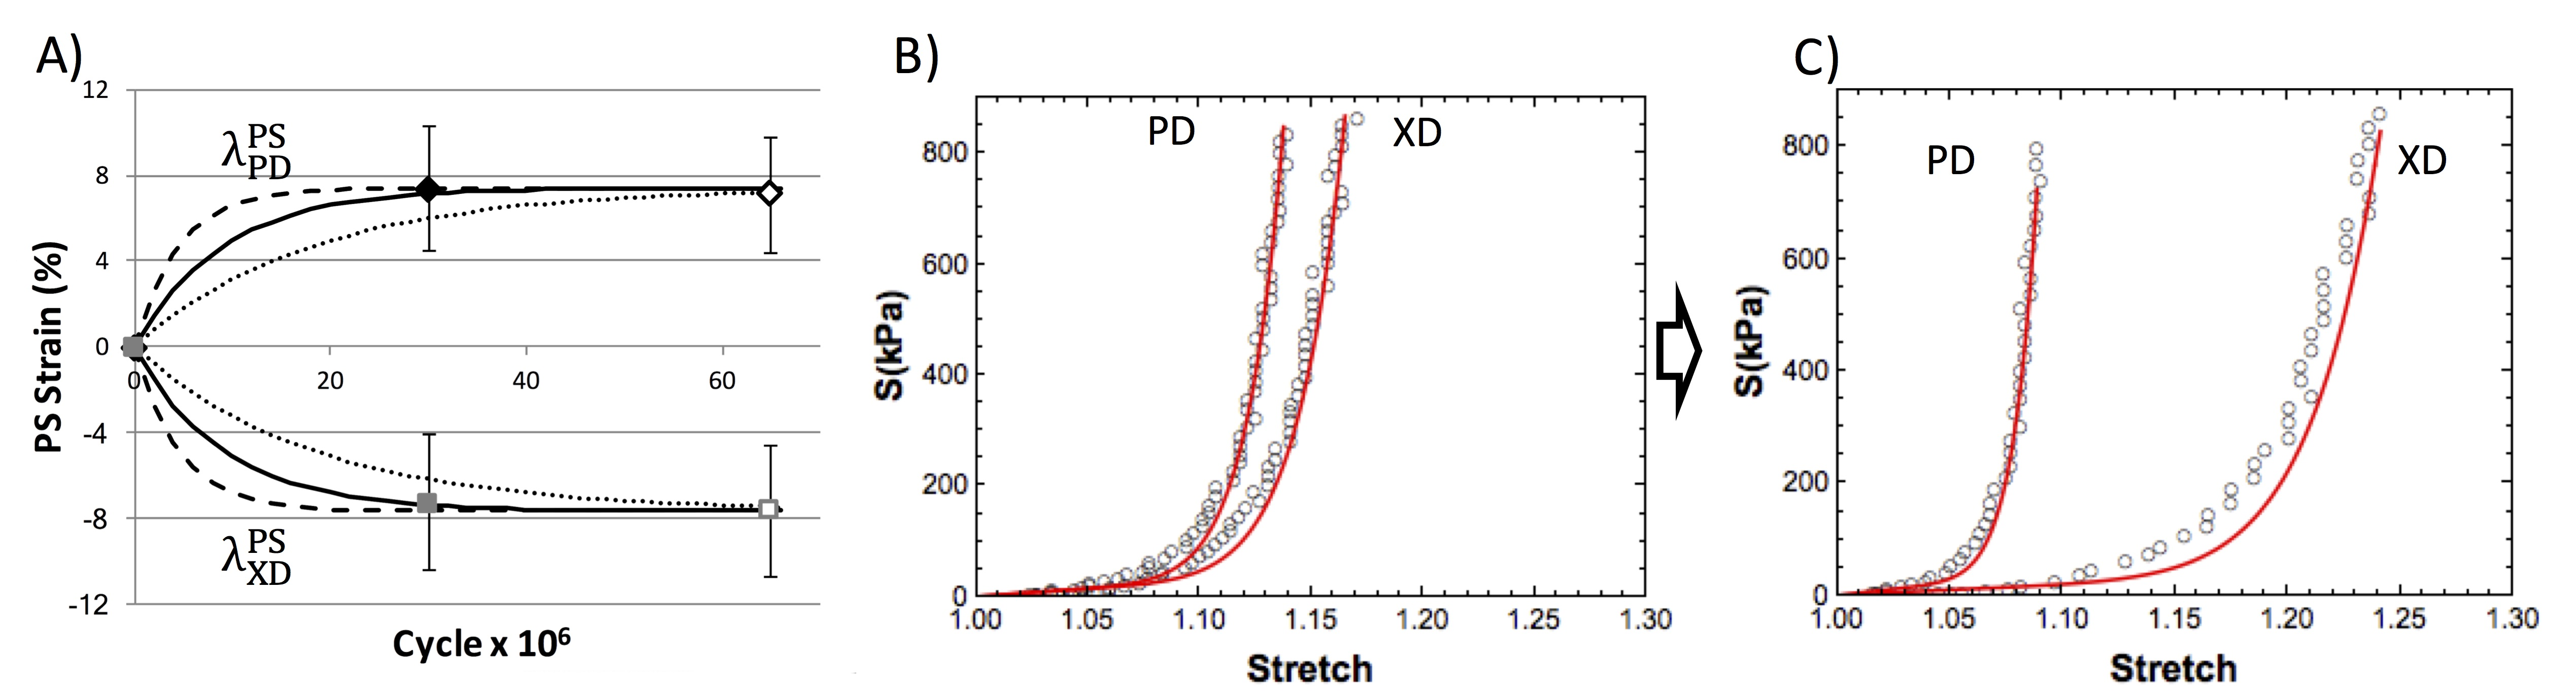
\includegraphics[width=0.75\paperwidth]{Images/chapter4/figure14}}
\caption{A) The model fit for the permanent set deformation at both 20 and 50 million cycles for the stress controlled XD cycled specimens. B) Comparison of the permanent set rate constant between the strain controlled and stress controlled specimens. C) The predicted permanent set deformation for the PD cycled specimens using the rate constant from fitting the XD cycled specimens. }
\label{fig:stressXDdef}
\end{figure}
\begin{figure}[hbt]
\centering
\centerline{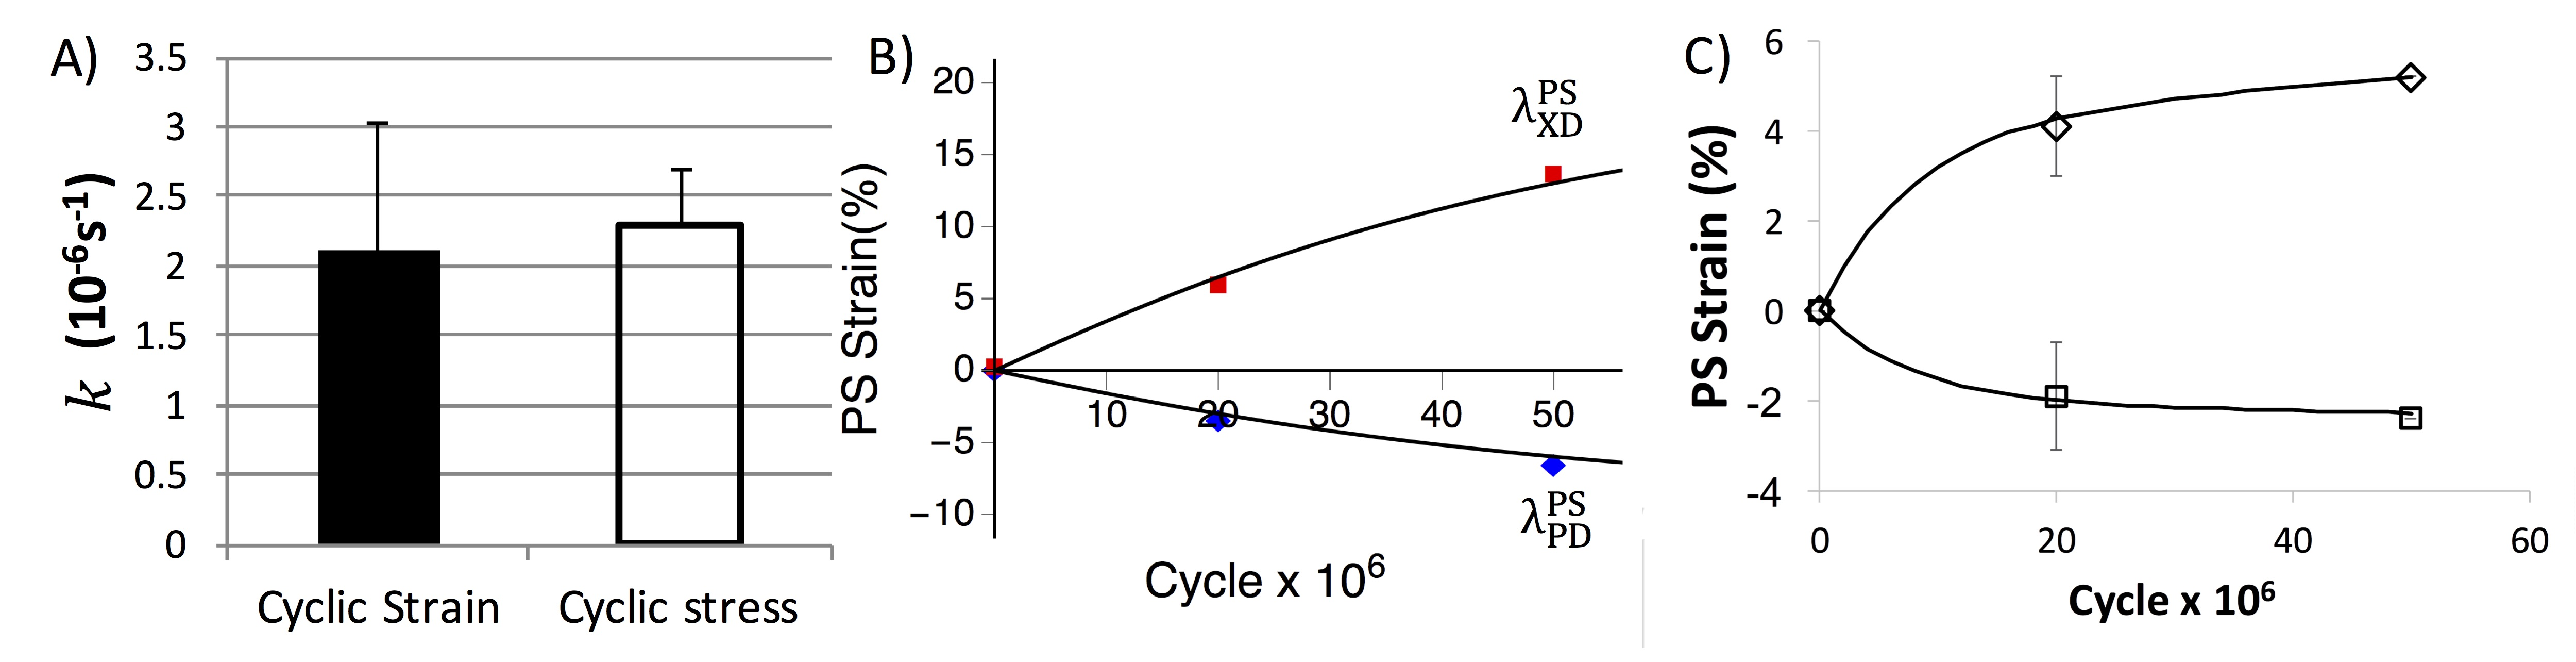
\includegraphics[width=0.75\paperwidth]{Images/chapter4/figure15}}
\caption{A) Best fit of the mechanical response at 0 cycle for the material parameters ($r^2 = 0.98$). The predicted mechanical response for the representative PD cycled specimen at B) 20 ($r^2 = 0.87$) and C) 50 million cycles. ($r^2 = 0.82$)}
\label{fig:stressPDmech}
\end{figure}

\subsection{Parametric study results}
	By extending the cycling duration in the parametric study, we found that the permanent set deformation reaches an assymptote after approximately 70 million cycles when loading along the PD. 
	This threshold slightly exceeds the lower bound for collagen recruitment. 
	We estimate that around 2.6\% of collagen fiber are recruited when the permanent set deformation reaches this threshold (Fig. \ref{fig:parametric}). 
	This suggests that collagen fibers are limiting the maximum change in geometry that can occur, and that the lower bound of the collagen fiber recruitment can serve as an estimated bound for the change in geometry due to the permanent set effect in BHVs, as collagen fibers start resisting further deformation of the exogenously crosslinked the matrix. Once this bound is exceed, some collagen fibers can exist perennially in an extended state. This could be a potential mechanism in exacerbating the rate of damage to the collagen fiber architecture. 

\begin{figure}[hbt]
\centering
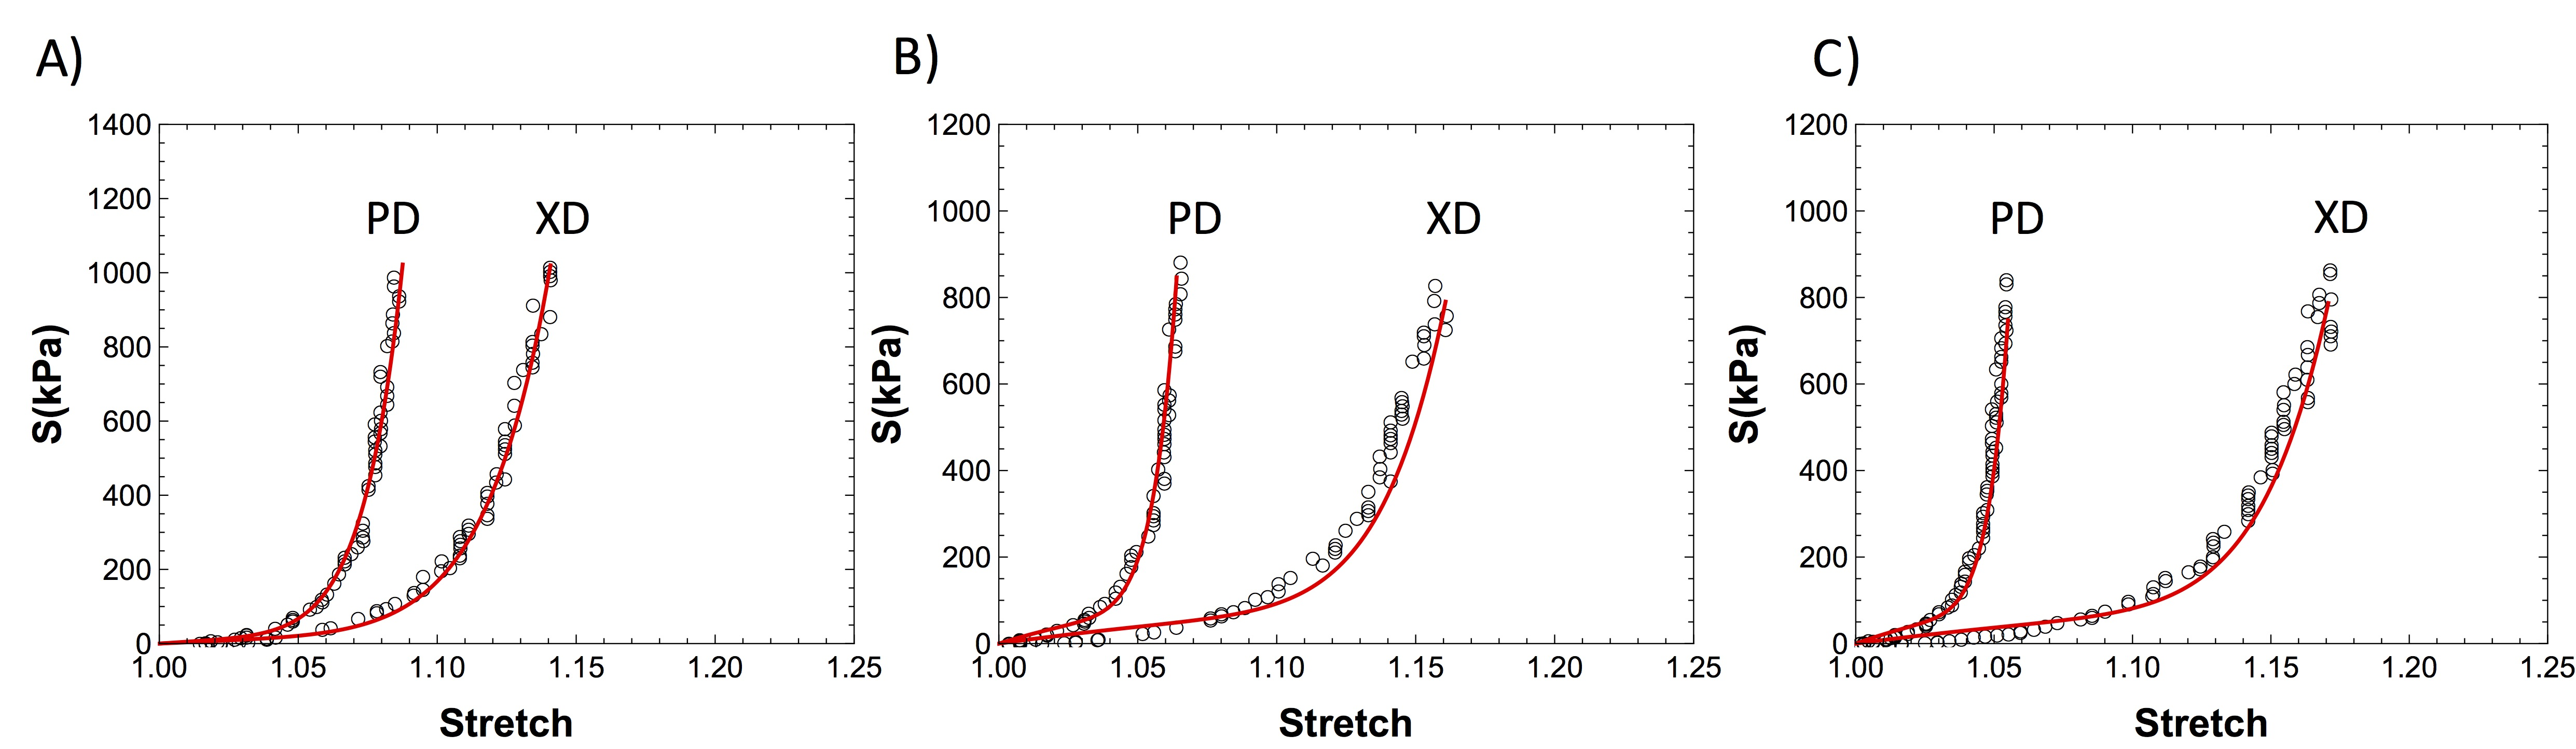
\includegraphics[width=0.35\paperwidth]{Images/chapter4/figure16}
\caption{The results of the parametric study. The red solid line shows the lower bound for the collagen fiber slack stretches and the red dashed line show the approximate cycle when the permanent set stretches reach an assymptote.}
\label{fig:parametric}
\end{figure}